A atividade de elicitação de requisitos tem o objetivo de entender junto ao cliente as necessidades do negócio e identificar as características do sistema. É importante ressaltar que essa é uma fase crucial no processo de software, e para se ter êxito serão utilizadas algumas técnicas de elicitação.

Por ser um processo muita das vezes complexo, o Sommerville cita algumas dificuldades para o processo de elicitação de requisitos, que são elas:

1- Os stakeholders muitas das vezes não sabem o que querem do sistema. Eles entendem o sistema de maneira geral, e encontram muitas dificuldade em articular as especificidades do sistema, podendo fazer pedidos não realistas por não saberem o custo de suas solicitações.

2- Os stakeholders usam termos técnicos que imprimem um conhecimento implícito e cabe aos engenheiros de requisitos conhecerem a área de conhecimento do cliente.

3- Diferentes stakeholders tem em mente diferentes requisitos, dificultando o trabalho dos engenheiros, que precisam identificar as semelhanças e os pontos conflitantes dos requisitos.

4- Fatores hierárquicos e políticos afetam o sistema. Eles podem fazer com que gerentes definam requisitos para aumentar seu poder de influência dentro da organização.

5- A adaptabilidade do sistema é um fator muito importante. Dentro do ambiente econômico e dos negócios a mutabilidade dos requisitos é inevitável, podendo mudar durante o processo de elicitação.

O Sommerville aborda a elicitação de requisitos a princípio de maneira mais simplificada, tendo como abordagem um modelo interativo incremental, com feedbacks contínuos entre as atividades. Que são elas:

“Compreensão do domínio: Os analistas devem desenvolver sua compreensão
do domínio da aplicação;

Coleta de requisitos: É o processo de interagir com os stakeholders do sistema
para descobrir seus requisitos. A compreensão do domínio se desenvolve mais durante essa atividade;

Classificação: Essa atividade considera o conjunto não estruturado dos
requisitos e os organiza em grupos coerentes;

Resolução de conflitos: Quando múltiplos stakeholders estão envolvidos, os
requisitos apresentarão conflitos. Essa atividade tem por objetivo solucionar
esses conflitos;

Definição das prioridades: Em qualquer conjunto de requisitos, alguns serão mais importantes do que outros. Esse estágio envolve interação com os stakeholders para a definição dos requisitos mais importantes;

Verificação de requisitos: Os requisitos são verificados para descobrir se estão completos e consistentes e se estão em concordância com o que os stakeholders desejam do sistema.”

Ratificando a informação supracitada, o modelo abaixo mostra uma imagem referente ao processo de levantamento e análise de requisitos.

\FloatBarrier
\begin{figure}[!htpd]
		\centering
		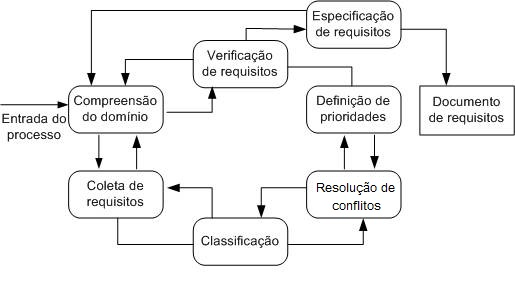
\includegraphics[scale=1.0]{figuras/analise}
		\label{img:a}
		\caption{Processo de levantamento e análise de requisitos}
\end{figure}
\FloatBarrier


\section {Técnicas de elicitação de requisitos}

\subsection {Levantamento orientado a ponto de vista}

Em sistemas de diferenciados tamanhos, tanto pequenos, como médios, como grandes existem diferentes pontos de vista. Por exemplo, em um sistema de caixa automático bancário os clientes do banco vão receber os serviços do sistema, os representantes de outros bancos que tem parceria no uso do caixa automático, gerentes de agência que obtém dados do sistema, administradores de banco de dados que vinculam os dados da conta do cliente com os dados que vão ser mostrados no caixa automático, gerentes de segurança bancária, que vão assegurar a integridade do sistema, o departamento de marketing para fazer divulgação dos produtos do banco e os responsáveis pela manutenção do caixa automático, que vão garantir a boa integridade do sistema. A relação supracitada evidencia que em um sistema relativamente simples, os pontos de vista são diferentes, contudo não independentes, existindo muitos pontos de interseção entre eles, bem como pontos conflitantes e/ou de duplicidade.

Na elicitação baseada em pontos de vista, ela reconhece esses diferentes pontos de vista para a estruturação e organização dos processos de elicitação de requisitos, e também dos requisitos. As vantagens do levantamento por ponto de vista é uma visão mais ampla no sistema, além de uma facilidade maior de identificar conflitos entre os requisitos que os stakeholders propuseram.

Existem abordagens de elicitações por pontos de vista como SADT (Ross, 1977; Schoman e Ross 1977) e o CORE (Mullery, 1979) que citam a elicitação de requisitos como uma fonte de dreno de dados, onde os pontos de vista vão ser responsáveis pela parte que produz ou consome dados. Esses dois métodos são os primeiros a propor pontos de vista explícitos.

Outros autores definem a análise por ponto de vista como um framework de representação, onde o ponto de vista é considerado um tipo particular de modelo de sistema \cite {gotel}. Podemos exemplificar essa citação com diferentes engenheiros fazendo um diagrama de sequência, e outros fazendo um diagrama de classes, cada um dos diagramas feitos vai identificar uma abordagem diferente do sistema.

\cite {kotonya} definem o levantamento orientado a ponto de vista como um receptor de serviços, onde os pontos de vista são externos ao sistema, e do ponto de vista recebem serviços.

Apesar de existirem diferentes métodos de análises de pontos de vista citados acima, nenhum deles é adequado para a estruturar uma elicitação de requisitos, porque não existe nenhuma relação simples entre os pontos de vista e os stakeholders.

Em contraposição, sistemas interativos visam integrar da melhor forma os stakeholders. Consequentemente uma abordagem mais eficaz.

\subsection {Prototipagem}

Os protótipos são úteis para a elicitação de requisitos, porque os usuários poderão experimentar com o sistema e mostrar os pontos fortes e fracos do sistema. Eles terão algo concreto para criticar. \cite{castro}

Atualmente existem dois tipos de prototipagem, a descartável a e evolucionária. A descartável procura ajudar na na elicitação e no desenvolvimento dos requisitos, os requisitos que vão prototipados são aqueles que os clientes tem
mais dificuldades para especificar, os requisitos bem interpretados não precisam de implementação.

Já a prototipação evolucionária tem como objetivo a entrega rápida de um sistema funcional para o cliente, assim, os requisitos que vão ser implementados serão aqueles que estão bem definidos pelo cliente.
Entre os benefícios da prototipagem podemos ressaltar alguns pontos, que são eles:

\begin{itemize}
\item O protótipo permite que os usuários experimentem e descubram o que eles realmente necessitam para suportar o trabalho deles.
\item Estabelece viabilidade e utilidade antes que altos custos de desenvolvimento tenham sido realizados.
\item A prototipagem força estudos detalhados dos requisitos, apontando inconsistências e omissões.
\end{itemize}

\subsection{JAD}

O JAD é uma metodologia aplicada pela IBM em 1977, e implantada no Brasil em 1982. é uma técnica baseada em em reuniões, que permite que todos tenham um visão do produto. Sua principal finalidade é acelerar o desenvolvimento de software, essa metodologia está sendo empregada em amplas áreas de projeto \cite {camila}.

Os princípios da metodologia é a realização de dinâmicas em grupo, utilização de recursos audiovisuais, analisar o projeto de forma completa (top-down), garantindo que todas as partes do processo sejam abrangidas, utilização de uma documentação padrão, para que possa ser entendida por todos os membros do grupo.

O JAD se divide em duas etapas: Planejamento e projeto, onde no planejamento ocorre a elicitação dos requisitos, e na fase de projeto ocorre a gerência e desenvolvimento do sistema. Cada etapa possui três fases: Adaptação, sessão e finalização, onde na adaptação se prepara o material utilizado nas reuniões, as sessões seriam as sessões de reuniões, e na finalização, converte-se os documentos extraídos em documentos.

Os benefícios do JAD são o trabalho em equipe, maior produtividade e qualidade, além do baixo custo.

\subsection{Brainstorming}

Neste tipo de reunião, representantes de diferentes grupos de interessados engajam-se em uma discussão informal para gerar rapidamente tantas
ideias quanto possível, sem focar a atenção em nenhuma delas(Aurum; Wohlin, 2005).

Como o nome já diz, o processo supracitado é um período de Brainstorming, se traduzirmos ao pé da letra: tempestade cerebral. Em geral esse período de tempestade cerebral tem como objetivo resolver um grande número de questões, ou tomar decisões. Geralmente essa técnica é usada para se obter uma visão preliminar do sistema. Uma das grandes vantagens do Brainstorming, é que ao permitir a livre expressão dos componentes da reunião, conseguem chegar soluções criativas e inovadoras para o sistema.

\subsection{Entrevista}

A entrevista visa identificar o problema, propor a solução, negociar os aspectos de abordagem e identificar um conjunto preliminar  de requisitos do projeto. \cite{moraes}

\begin{itemize}
\item As entrevistas serão conduzidas com a participação dos engenheiros de software e outros interessados.
\item A agenda de entrevistas deve possibilitar uma entrevista que cubra todos os pontos importantes,  e abra espaço para o fluxo de novas ideias.
\item Deve haver  um controle da reunião através de um plano de entrevista, para que não haja uma dispersão do conteúdo pertinente ao entrevistador.
\end{itemize}

\section{Elicitação Escolhida}

As técnicas são utilizadas para identificar os requisitos conscientes, inconscientes e subconscientes dos stakeholders. Cada projeto possui características específicas, e por isto, algumas técnicas são melhor aplicadas em determinado contexto. Segundo \cite{pohl} os fatores mais influentes para a escolha das técnicas são:

\begin{itemize}
\item Distinção entre os requisitos conscientes, inconscientes e subconscientes a serem elicitados.
\item As restrições em termos de tempo e de orçamento, bem como de disponibilidade dos stakeholders.
\item A experiência do engenheiro de requisitos com determina técnica de elicitação.
\item As oportunidades e risco do projeto.
\end{itemize}

Levando em consideração esses aspectos, foi feita uma análise do contexto para o levantamento de requisitos, percorrendo e analisando as diversas técnicas que são usadas atualmente, como o levantamento orientado a ponto de vista, etnografia, prototipagem, entrevista, questionário, brainstorming e JAD.

Partindo do princípio que já existe uma parte do nosso software pronto, e que a cliente conhece bem os requisitos e tem noções de desenvolvimento de software, técnicas como JAD, apesar de promover a cooperação, o trabalho em grupo e o entendimento, acabam não se adaptando, devido sua metodologia ser baseada na criação e na resolução de problemas, onde os desenvolvedores ajudam os usuários do sistema a criarem problemas e eles mesmos proporem soluções. \cite{moraes}

O Brainstorming é uma técnica que no começo suas ideias não parecem convencionais, mas são encorajadas, estimulando frequentemente os participantes para a elaboração de soluções criativas. Mas a exploração de novas ideias não se aplica ao nosso caso, porque a ideia do software já existe. \cite{moraes}

A prototipagem parte do pressuposto de fazer protótipos para a validação do cliente, implementando os aspectos críticos do sistema. Porém, já existe um protótipo validado pela cliente, e esta técnica ao ser adotada geraria um retrabalho.

O Sommerville recomenda a elicitação por pontos de vista. Apesar dessa elicitação ser bem respaldada acima por diversos autores de renome na elicitação de requisitos, como Finkelsten, Schoman, Ross, Mullery, Nuseibeh e Kotonya, os pontos de vista de diferentes stakeholders são necessários para a definição de requisitos, e atualmente temos apenas a visão de uma pessoa do grupo, e consequentemente não temos recurso necessário para a aplicação.

Após a análise destas ferramentas, chegou-se a conclusão que a  técnica melhor ser aplicada a este projeto é a entrevista. Ela se enquadra melhor visto que o projeto já teve uma parte iniciada e que o grupo não possui limitações em termos de disponibilidade, distância, podendo assim serem feitas reuniões semanalmente utilizando a técnica de entrevista.
